\documentclass[]{article}
\usepackage[utf8]{inputenc}
\usepackage[sumlimits]{amsmath}
\usepackage{amssymb}
\usepackage{color,array,graphics}
\usepackage{hyperref}
\usepackage{enumerate}
\usepackage{graphicx}
\usepackage{amsmath, amsthm, amssymb}
\usepackage[shortlabels]{enumitem}
\usepackage[english]{babel}
\usepackage{tikz}
\usepackage{caption}
\usepackage{subcaption}
\usepackage{cellspace}
\setlength\cellspacetoplimit{4pt}
\setlength\cellspacebottomlimit{4pt}

\newcommand\cincludegraphics[2][]{\raisebox{-0.1\height}{\includegraphics[#1]{#2}}}

\setlength{\textheight}{8.5in}
\setlength{\textwidth}{6.5in}
\setlength{\oddsidemargin}{0in}
\setlength{\evensidemargin}{0in}
\voffset0.0in

\def\OR{\vee}
\def\AND{\wedge}
\def\imp{\rightarrow}
\def\math#1{$#1$}
\def\mand#1{$$#1$$}
\def\mld#1{\begin{equation}
#1
\end{equation}}
\def\eqar#1{\begin{eqnarray}
#1
\end{eqnarray}}
\def\eqan#1{\begin{eqnarray*}
#1
\end{eqnarray*}}
\def\cl#1{{\cal #1}}

\DeclareSymbolFont{AMSb}{U}{msb}{m}{n}
\DeclareMathSymbol{\N}{\mathbin}{AMSb}{"4E}
\DeclareMathSymbol{\Z}{\mathbin}{AMSb}{"5A}
\DeclareMathSymbol{\R}{\mathbin}{AMSb}{"52}
\DeclareMathSymbol{\Q}{\mathbin}{AMSb}{"51}
\DeclareMathSymbol{\I}{\mathbin}{AMSb}{"49}
\DeclareMathSymbol{\C}{\mathbin}{AMSb}{"43}

\title{Assignment 3}
\author{Batch Size of 3}

\begin{document}

\maketitle

\clearpage
\section{CLIP}

\subsection{Dataset}

In this iteration of the homework, our dataset consists of various objects and items contained in a kitchen. As you can see, these objects are not common household items, but those are included as well. The inclusion of the items are meant to serve as a way to differentiate common used items and uncommon items that it might not correlate. For instance, a fork and spoon may have a high correlation, but probably not a mop bucket and fork. Here is the dataset with the captions that our team agreed on:

\begin{figure}[h]
    \centering
    \begin{subfigure}[b]{0.2\textwidth}
        \centering
        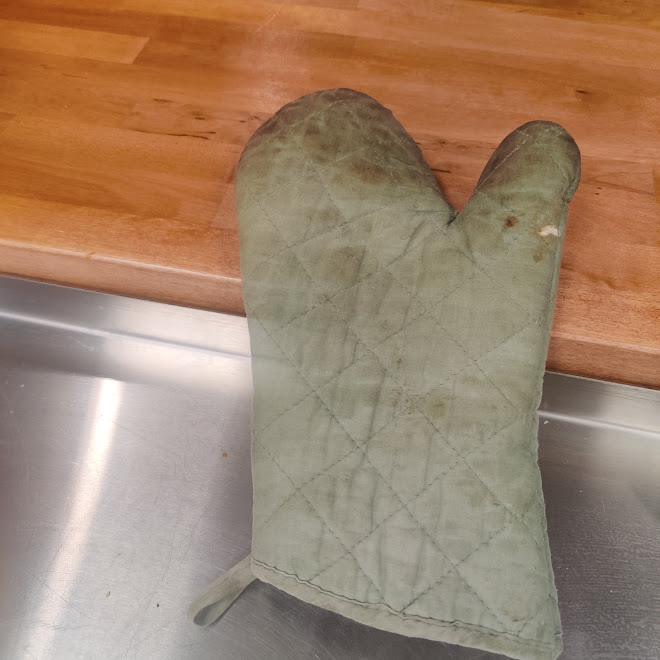
\includegraphics[width=\textwidth]{dataset/0.jpg}
        \caption{oven mitt on the counter}
    \end{subfigure}
    \begin{subfigure}[b]{0.2\textwidth}
        \centering
        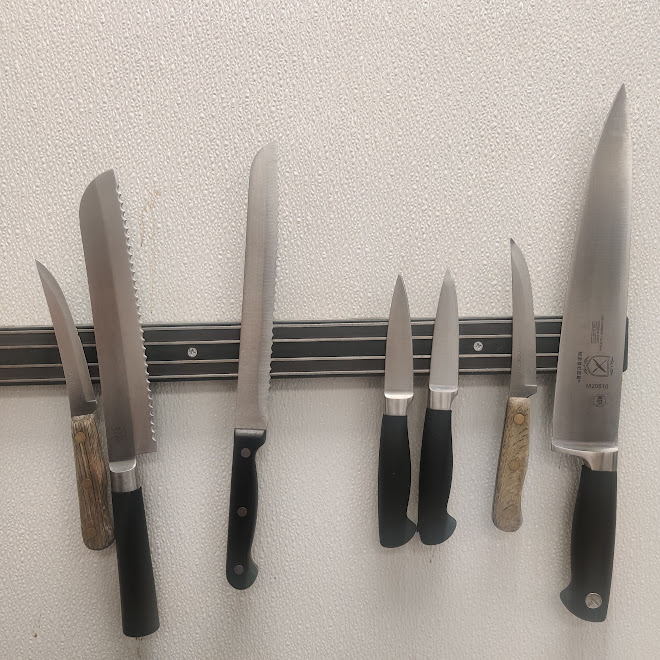
\includegraphics[width=\textwidth]{dataset/1.jpg}
        \caption{knives on the magnetic knife rack}
    \end{subfigure}
    \begin{subfigure}[b]{0.2\textwidth}
        \centering
        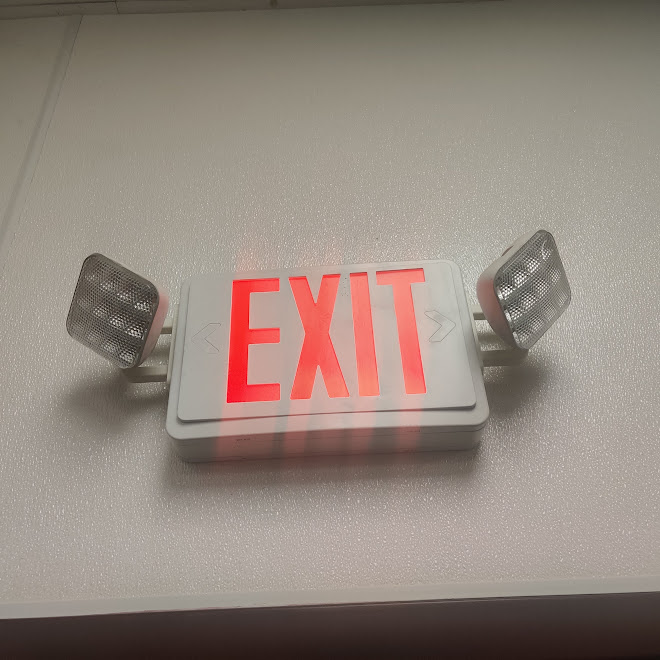
\includegraphics[width=\textwidth]{dataset/2.jpg}
        \caption{exit sign on the white wall with emergency lights}
    \end{subfigure}
    \begin{subfigure}[b]{0.2\textwidth}
        \centering
        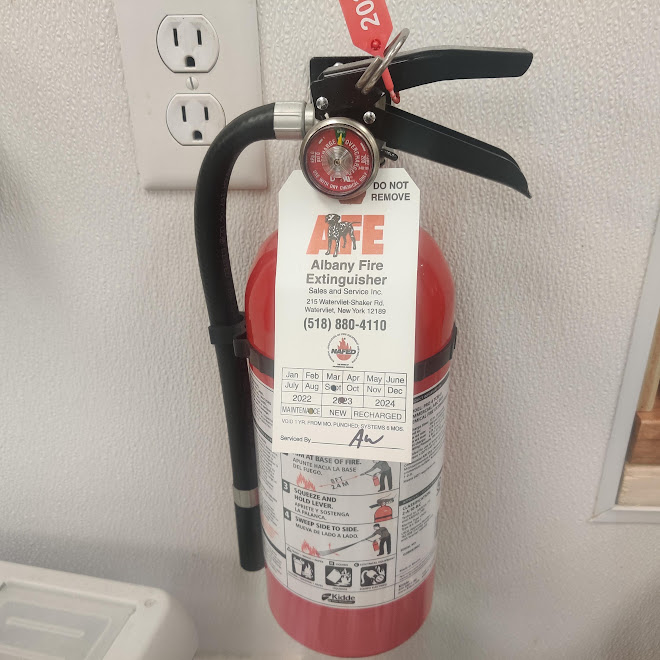
\includegraphics[width=\textwidth]{dataset/3.jpg}
        \caption{fire extinguisher on a white wall}
    \end{subfigure}
    \begin{subfigure}[b]{0.2\textwidth}
        \centering
        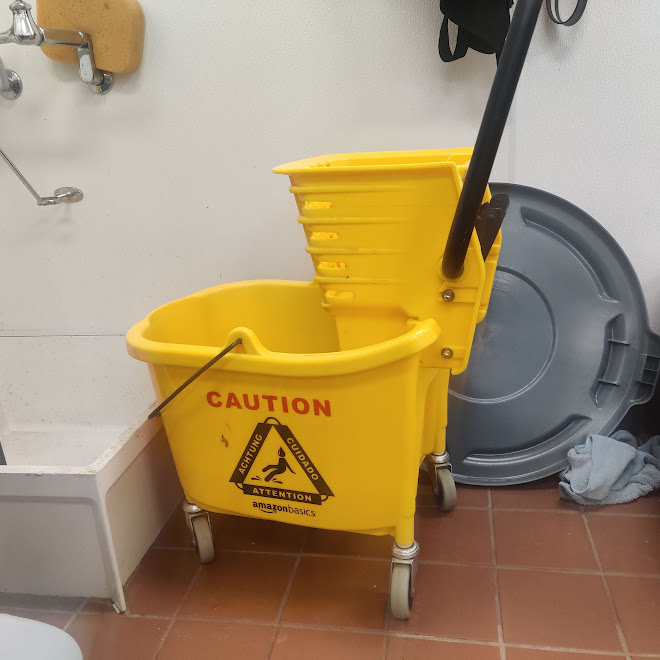
\includegraphics[width=\textwidth]{dataset/4.jpg}
        \caption{mopping bucket}
    \end{subfigure}
    \begin{subfigure}[b]{0.2\textwidth}
        \centering
        
\includegraphics[width=\textwidth]{dataset/5.jpg}
        \caption{butter knife on a wooden table}
    \end{subfigure}
    \begin{subfigure}[b]{0.2\textwidth}
        \centering
        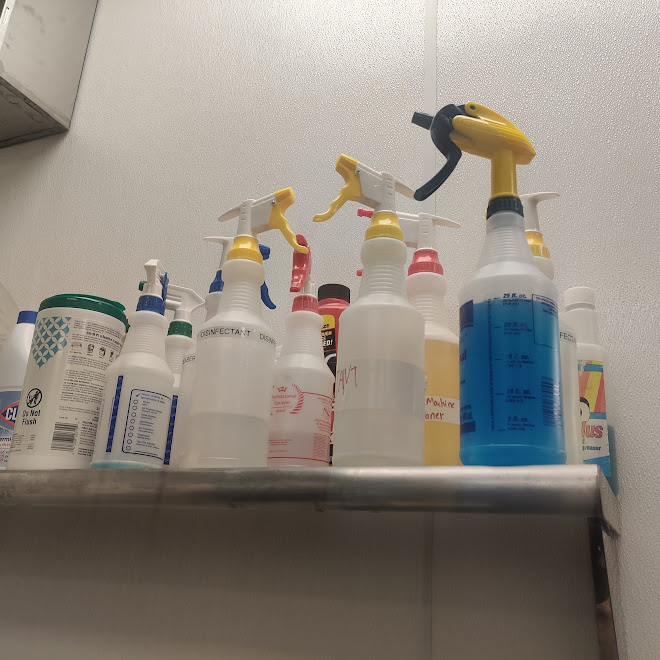
\includegraphics[width=\textwidth]{dataset/6.jpg}
        \caption{cleaning supplies on a shelf}
    \end{subfigure}
    \begin{subfigure}[b]{0.2\textwidth}
        \centering
        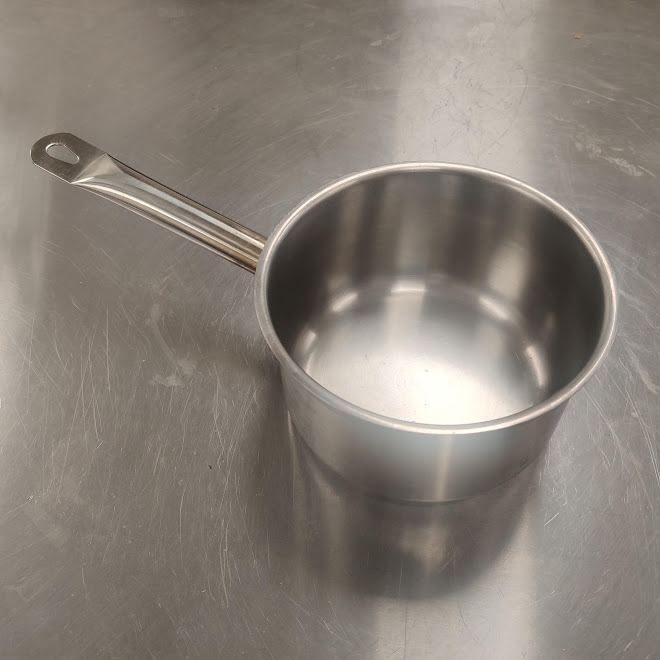
\includegraphics[width=\textwidth]{dataset/7.jpg}
        \caption{stainless steel saucepan on a metal counter}
    \end{subfigure}
    \begin{subfigure}[b]{0.2\textwidth}
        \centering
        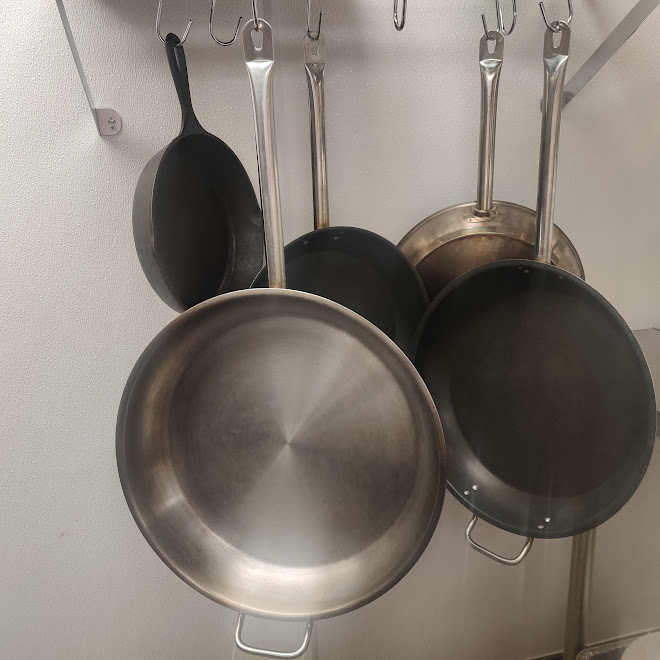
\includegraphics[width=\textwidth]{dataset/8.jpg}
        \caption{various pans hanging on a hook rack}
    \end{subfigure}
    \begin{subfigure}[b]{0.2\textwidth}
        \centering
        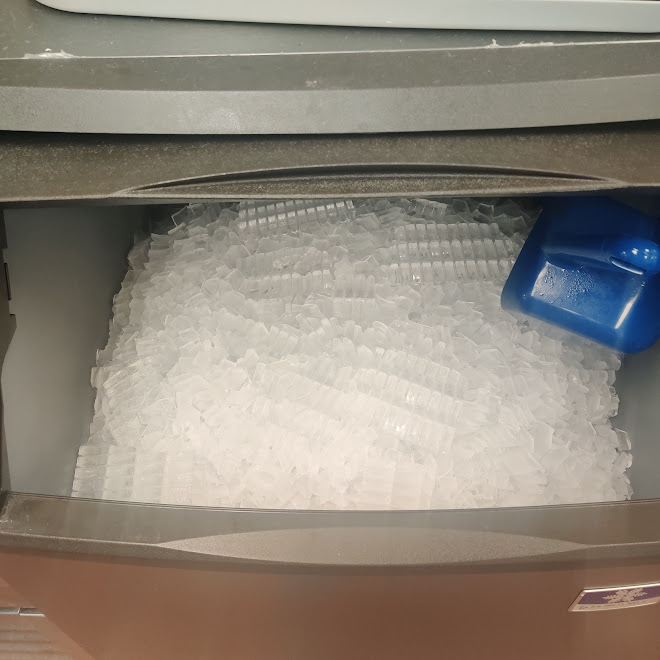
\includegraphics[width=\textwidth]{dataset/9.jpg}
        \caption{ice cubes in an ice maker}
    \end{subfigure}
    \caption{The dataset}
\end{figure}
\clearpage
% =========================================================
\subsection{(a) BERT Scores}
\begin{figure}[h]
    \begin{subfigure}[b]{0.5\textwidth}
        \centering
        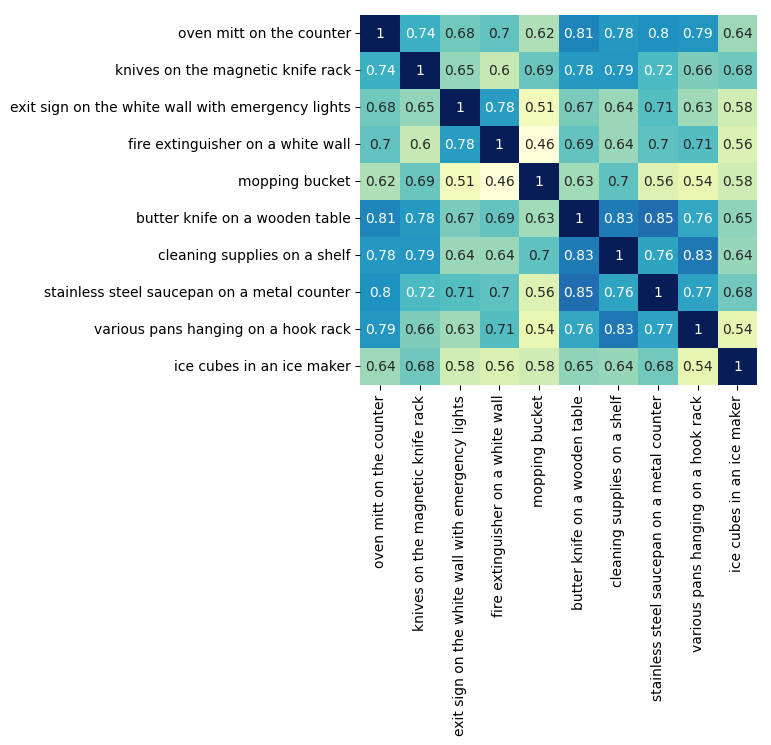
\includegraphics[width=\textwidth]{scores/bertscore.png}
        \caption{BERT similarity matrix}
    \end{subfigure}
    \begin{subfigure}[b]{0.5\textwidth}
        \centering
        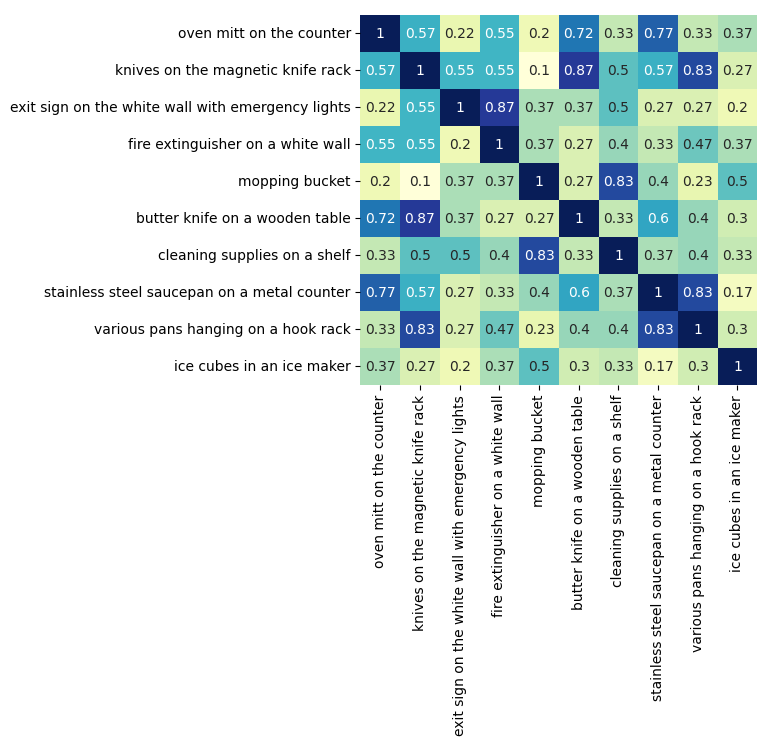
\includegraphics[width=\textwidth]{scores/userscores.png}
        \caption{User submitted similarity matrix}
    \end{subfigure}
\end{figure}

If we examine the similarity matrix for the text descriptions with BERT, we can confidently say that some similar items are similar as expected, and some items are not as similar compared to each other. Let us examine the similarity of objects considering only the BERT similarity matrix and our reasoning behind so. The similarity calculation for the user submitted score is based on mostly how we decide how a certain object is related to another. Some guidelines to these judgements include: use cases (how the object is used in that scenario and if they are used similarly), the situation in which the items are used in the same scenario (you use the fork and knife to eat food), the object material (metal, wooden), etc.\\
\\
\textbf{Examining the BERT similarity matrix}
\begin{itemize}
    \item \textbf{High scores with similar descriptions}
    \begin{itemize}
        \item stainless steel saucepan on a metal counter \& various pans hanging on a hook rack:
        \begin{itemize}
            \item these two items are very familiar, whereas one has one pan left out on a metal counter, the others are hanging on a rack. Since there is a direct correlation with stainless steel saucepan and various pans, there should be a high similarity between those items, and there is. If we look at the user submitted score, we also rated this very high, since the two descriptions include a class of kitchen objects (cooking utensils, which are pans).
        \end{itemize}
    \end{itemize}
    \item \textbf{Low scores with different descriptions}
    \begin{itemize}
        \item mopping bucket \& fire extinguisher on a white wall
        \begin{itemize}
            \item we can expect that a mopping bucket has nothing to do with a fire extinguisher and the results do show that it has the lowest common similarity. Compared with the user similarity score, we agreed on the fact that a mopping bucket is not very relevant to the fire extinguisher.
        \end{itemize}
    \end{itemize}
    \item
    \textbf{Average scores with average descriptions}
    \begin{itemize}
        \item fire extinguisher on a white wall \& oven mitt on the counter
        \begin{itemize}
            \item we can say that these items are similar if the case that it uses a similar other object (oven). So for instance, if the oven catches on fire, we need to use the fire extinguisher and we also use the oven mitt for the oven. However, the similarities end there and that is why we rated it an average score. BERT seemed to agree with us and also gave an average similarity score.
        \end{itemize}
    \end{itemize}
    
    \item 
    \textbf{High scores with different descriptions}
    \begin{itemize}
        \item cleaning supplies on a shelf \& oven mitt on the counter
        \begin{itemize}
            \item Cleaning supplies are generally used for cleaning surfaces and oven mitts are used to grab hot objects. Both are different items with different use cases, thus we rated the similarity very low. However, the textual descriptions are very similar, which did not agree with the human perspective.
        \end{itemize}
    \end{itemize}
    \item \textbf{Low scores with similar descriptions}
    \begin{itemize}
        \item various pans hanging on a hook rack \& knives on the magnetic knife rack
        \begin{itemize}
            \item Albeit, this is not a low score, but it is still less than average. We can say that both objects are metallic and hung up (in the same scenario). Which should make this more similar than different, and thus we rated both of the . However, BERT does not agree much with this and generally gives it a lower score. 
        \end{itemize}
    \end{itemize}
\end{itemize}
\clearpage
% =========================================================
\subsection{(b) CLIP scores}
The CLIP scores are displayed at Figure (3), and the relative score according to the maximum exact description to image score is at Figure (4). First and foremost, since all of the descriptions that we generated are the closest matched for CLIP, it means that the model worked correctly. CLIP correctly interpreted that the images and the descriptions that are provided with the images all match with each other. We can say that the similarity matrix generally works well with the text embeddings provided. 
\begin{figure}[h]
    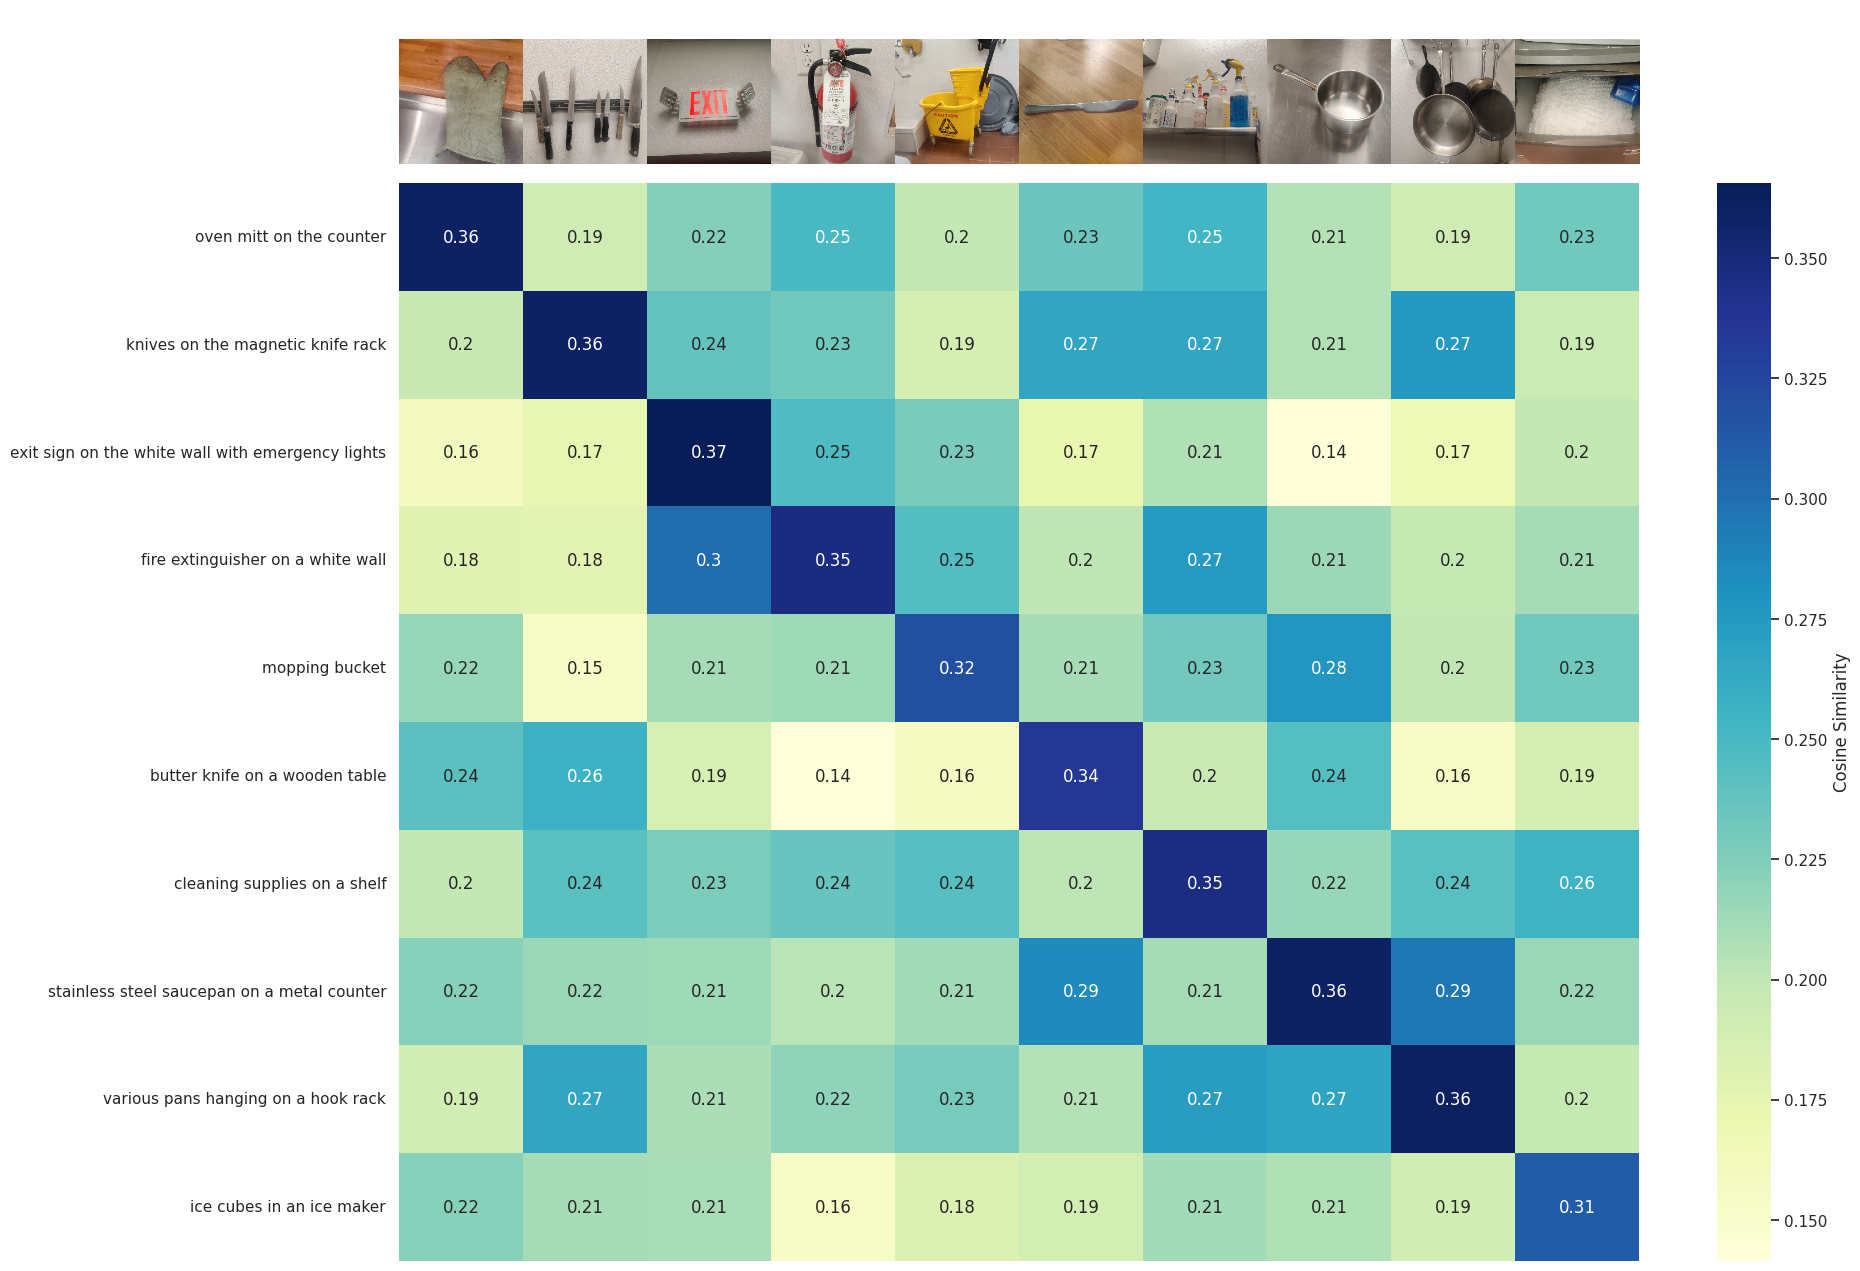
\includegraphics[width=18cm]{scores/clipscores.png}
    \caption{CLIP similarity matrix}
\end{figure}

Working with the same examples, the similarity between the various pans hanging on a hook rack and the saucepan image still have a higher similarity, which matched with our intuition. Moreover, the same goes for the butter knife on the table and the knives on the magnetic knife rack. On another note, it found that the knives hanging on the rack and pans hanging on the rack to have a high similarity score, which was not represented too much on the previous model (BERT). However, there are some differences, for instance, the cleaning supplies and mopping bucket should have a very high similarity score, since the mopping bucket needs the cleaning supplies to mop the floor. All in all, we can claim that this model generally works well with the provided texts/images.

\begin{figure}[h]
    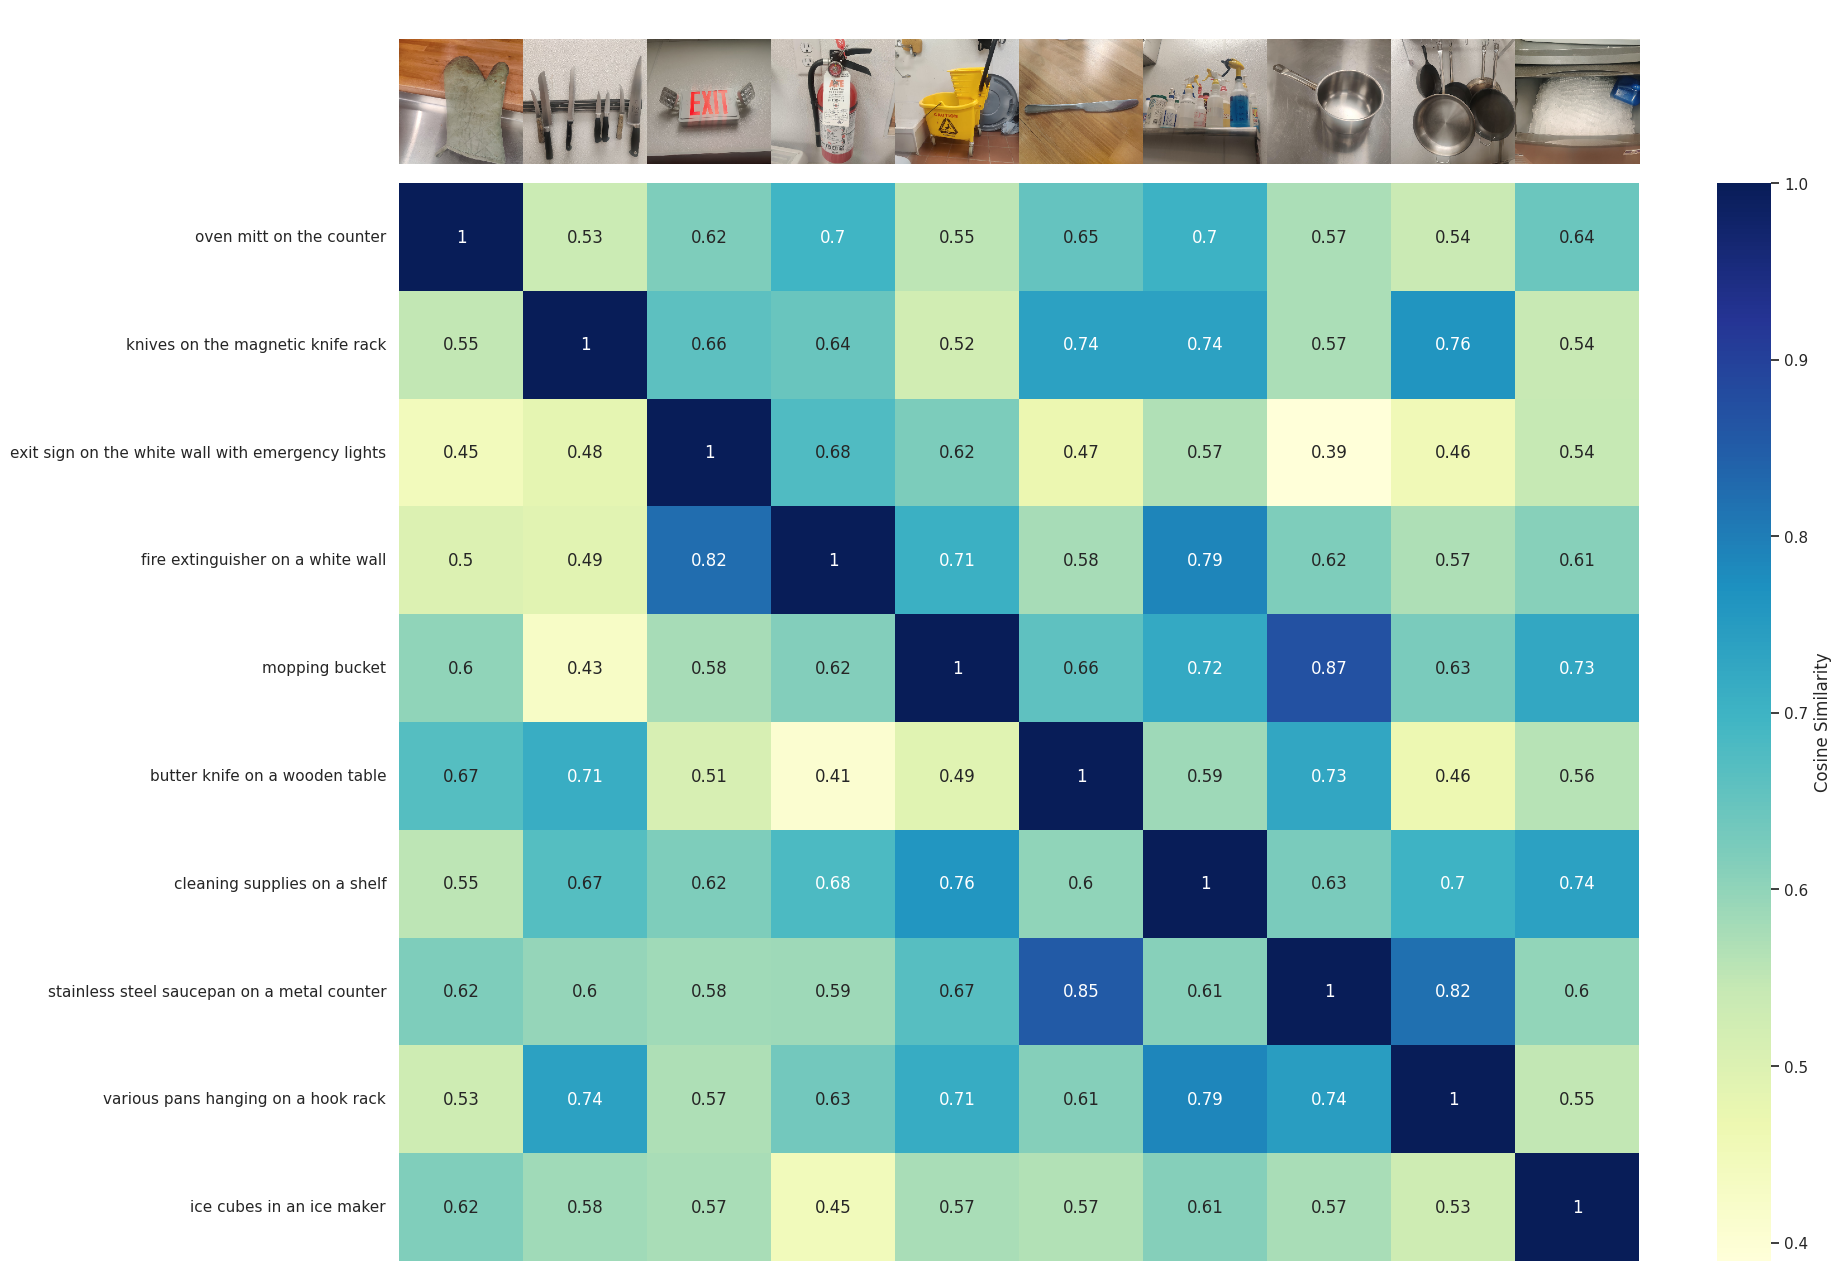
\includegraphics[width=18cm]{scores/cliprelativescores.png}
    \caption{CLIP similarity matrix relative to image/description CLIP score}
\end{figure}

\clearpage
\subsection{(c) Overall}
\begin{figure}[h]
    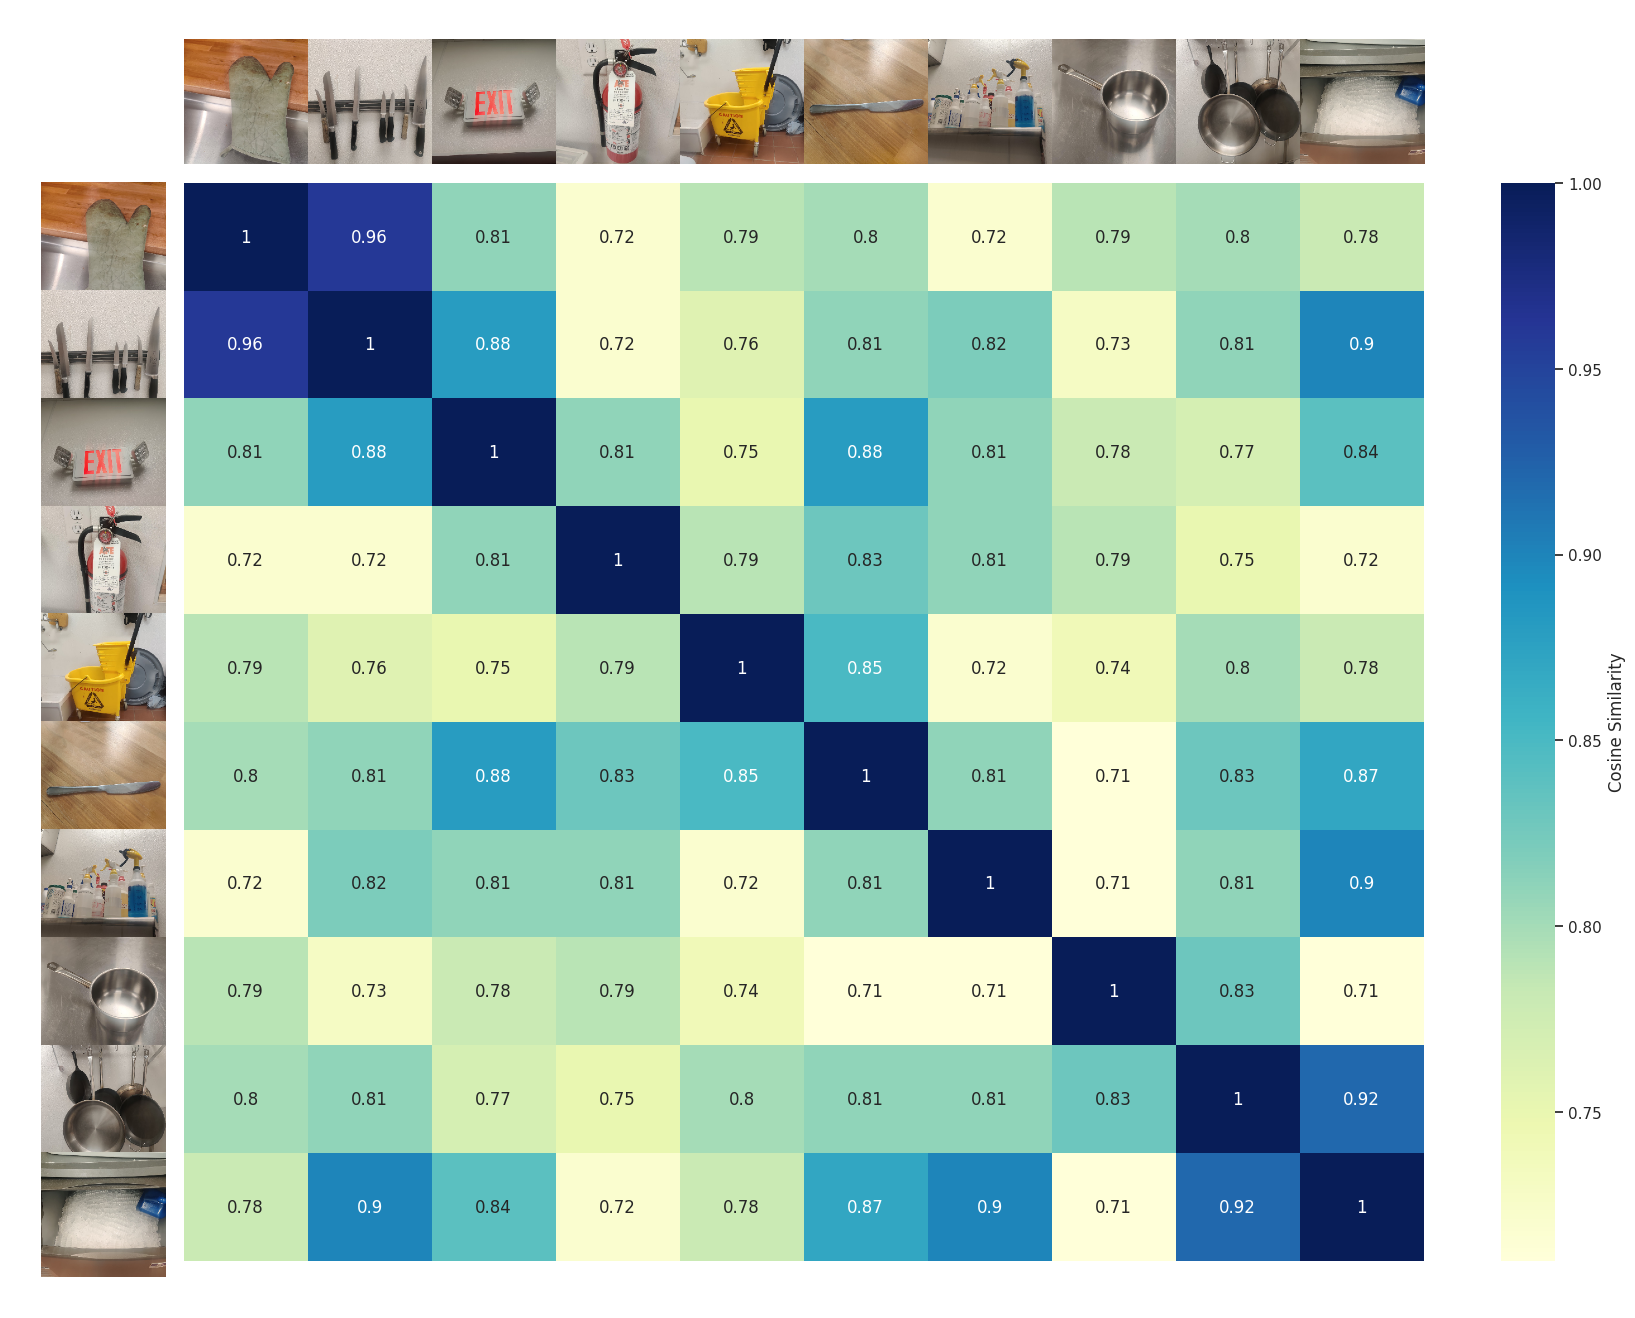
\includegraphics[width=16cm]{scores/lpipscore.png}
    \caption{LPIPS similarity matrix}
\end{figure}

If we examine the LPIPS prediction for the model, the pattern is very general and it doesnt seem like there are a lot of similarities between the model and what the images are. There are some images like the ice box and pots of pans hanging, that show very high similarity score, but not too relevantly close to each other in that instance. Same goes for the knives and the oven mitt, those scores are incredibly high, but the images dont match too well with each other. On the other hand, the saucepan and the various pans have a higher score, which does make sense since there is a large metallic pan/pot on the screen. We believe that out of all three models, LPIPS is slightly the worst, there is no general pattern that we expect from some images, and it seems like some values are random or vague. Moreover, it is hard to exactly tell if the images are coincidentally close to each other since the metric is very high for LPIPS. The other two models, BERT and CLIP have some examples where the similarity or dissimilarity makes sense, and some examples where it does not make sense. Thus, we think that the textual encoding for BERT and CLIP performs around the same for the given prompts/images for those models respectively, whereas LPIPS did worse.
% =========================================================
\subsection{CLIP experimentation: Image retrieval}
Image retrieval is a framework in which when a user gives an input text it will go through a dataset and search for all of the images that have the top 5th highest similarity embedding to text. In our use case, we added a food101 as our dataset. This dataset was subsetted to 2048 since it takes around 100 gb of memory to embed a total of 2048 images. Thus, if there are some similar images, that is due to the fact that the dataset is not as large as the entire food101 dataset. Although the dataset seems low, the results were good and varied. \\
\\
An example usage of this experiment is to have simple inputs like "beef" or "ramen" as text inputs, expecting images of beef or ramen as images to be displayed:
\begin{center}
    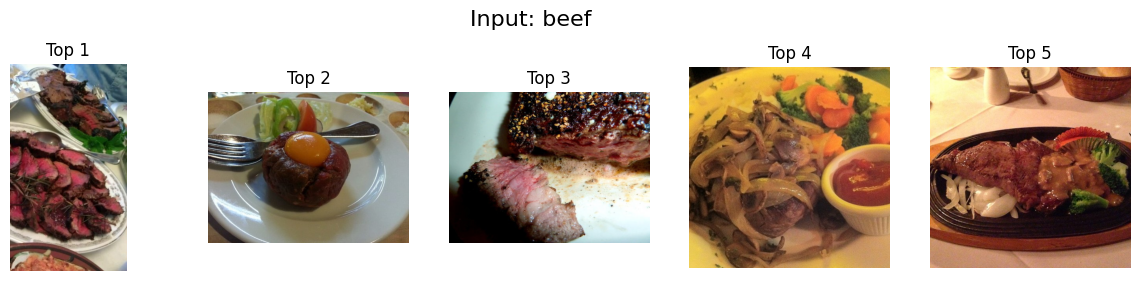
\includegraphics[width=14cm]{CLIP experiment/beef.png}
    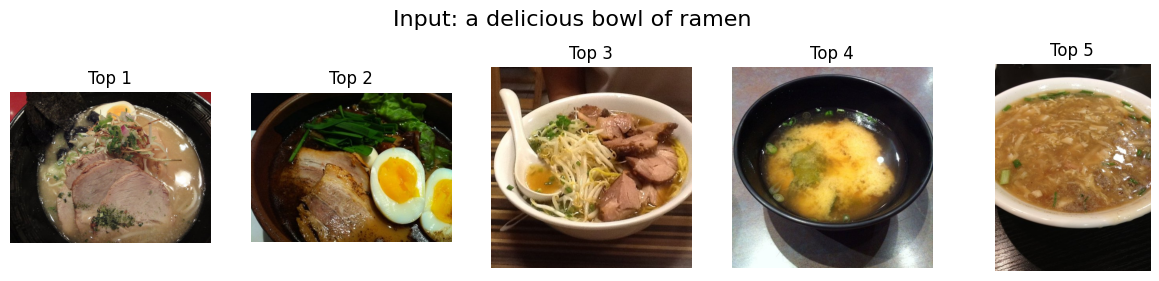
\includegraphics[width=14cm]{CLIP experiment/ramen.png}
\end{center}
food101 is a image classifier dataset with the given descriptions (class) of food. Thus, if we just only have inputs that are the class names for food101, it will should correctly return the class data for that food.\\
\centerline{\noindent\rule{16cm}{0.4pt}}\\
What if we want it to describe a specific cuisine and see how it will look like (i.e. will italian food include pasta?) 
\begin{center}
    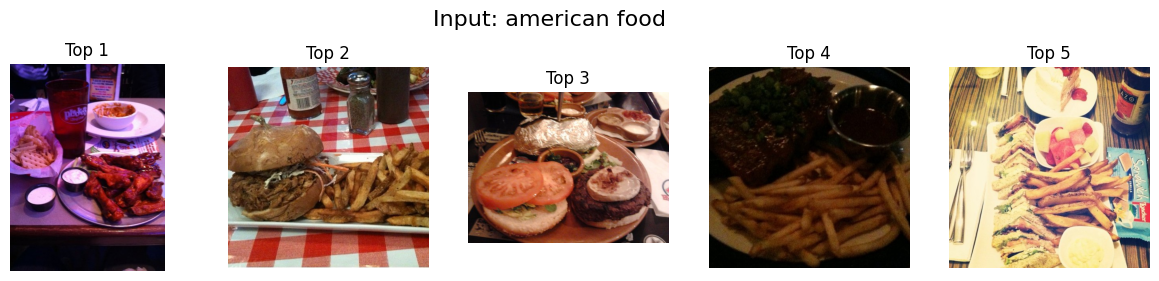
\includegraphics[width=14cm]{CLIP experiment/american.png}
    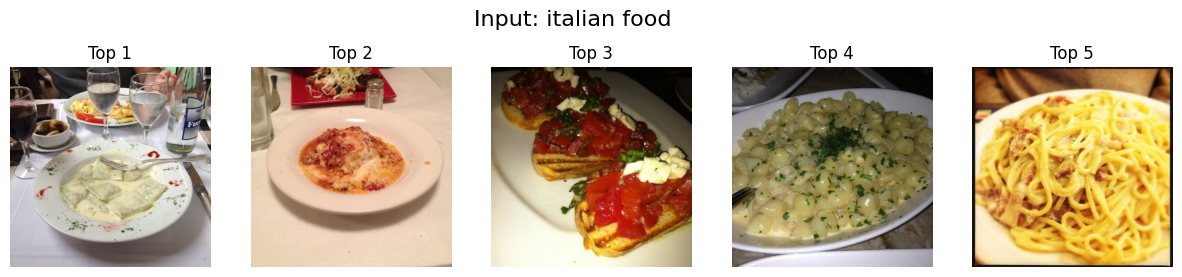
\includegraphics[width=14cm]{CLIP experiment/italian.png}
    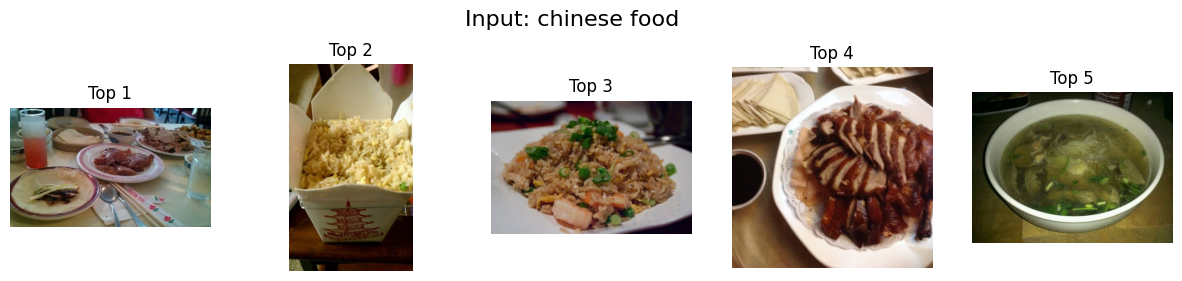
\includegraphics[width=14cm]{CLIP experiment/chinese.png}
\end{center}
as you can see there is a high correlation of what we think are "american foods" and "chinese foods" are included with the text description of that food. The italian food provided is also traditional and general depictions of italian food. Thus, the model was able to understand more than just the content of the food, but also the generalization of food.\\
\centerline{\noindent\rule{16cm}{0.4pt}}\\
Will it know based on the quantity of the food?
\begin{center}
    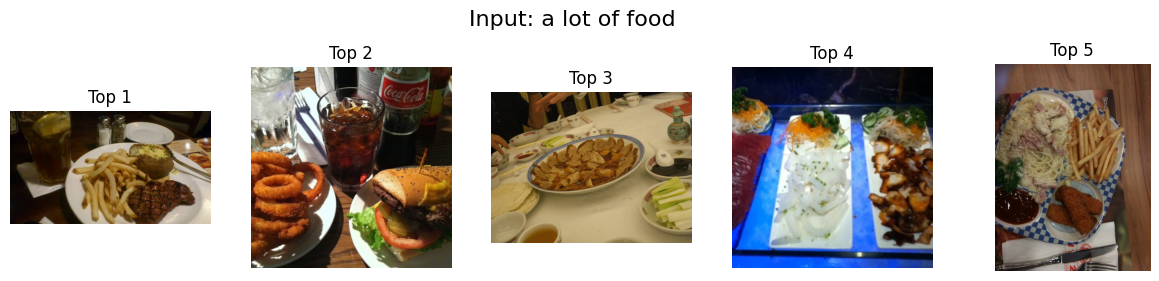
\includegraphics[width=14cm]{CLIP experiment/alotoffood.png}
    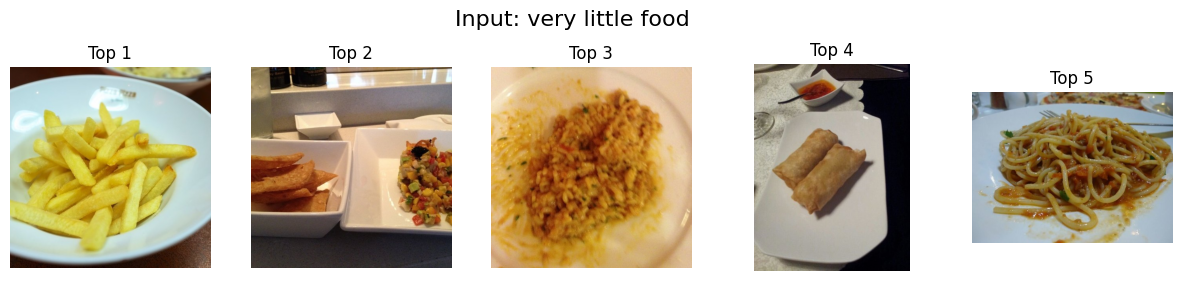
\includegraphics[width=14cm]{CLIP experiment/littlefood.png}
\end{center}
we can see that it does in fact know when there is a lot compared to very little food.

\centerline{\noindent\rule{16cm}{0.4pt}}
Since this is an open ended text based prompt, maybe we can use this to answer some deep food questions
\begin{itemize}
    \item Is cereal soup or is soup cereal? 
    \begin{center}
        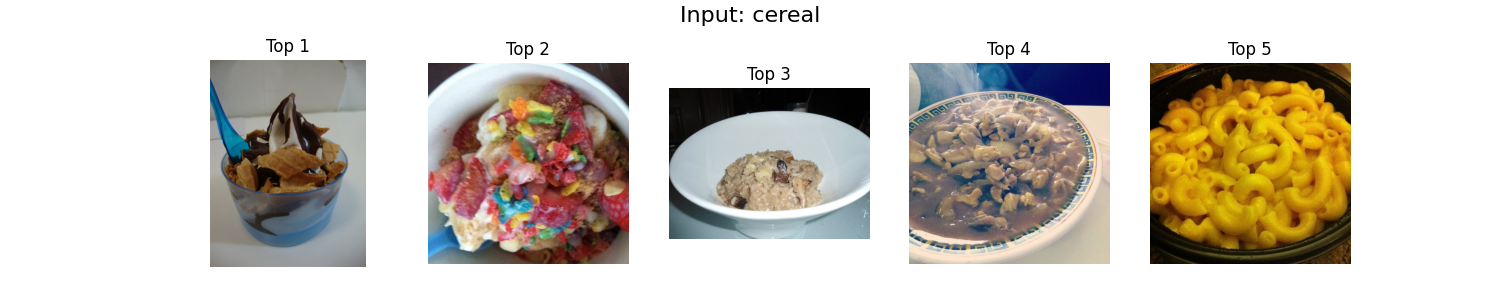
\includegraphics[width=14cm]{CLIP experiment/cereal.png}
        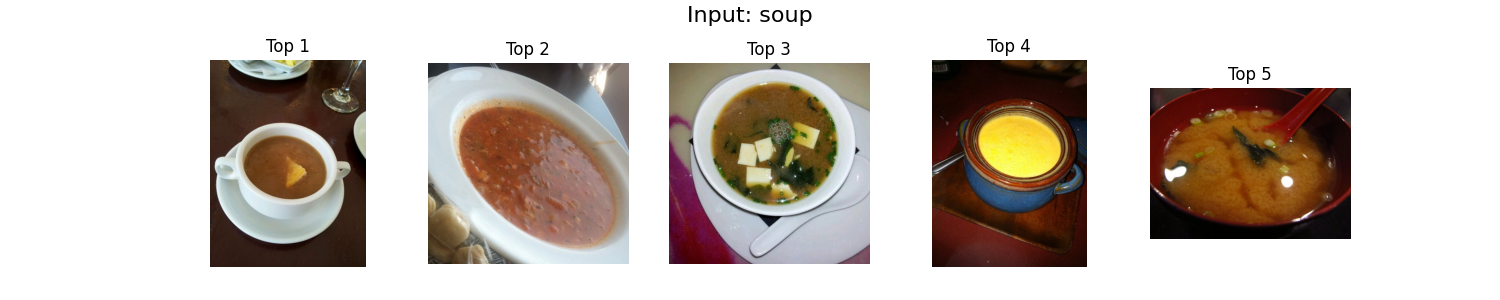
\includegraphics[width=14cm]{CLIP experiment/soup.png}
    \end{center}
    The real question is "is mac and cheese cereal?" (Beef Stroganoff was recognized as cereal as well, this probably means that in our subset, there was not enough examples of cereal)
    \item What do we consider the \textbf{BEST} food compared to the \textbf{WORST} food?
    \begin{center}
        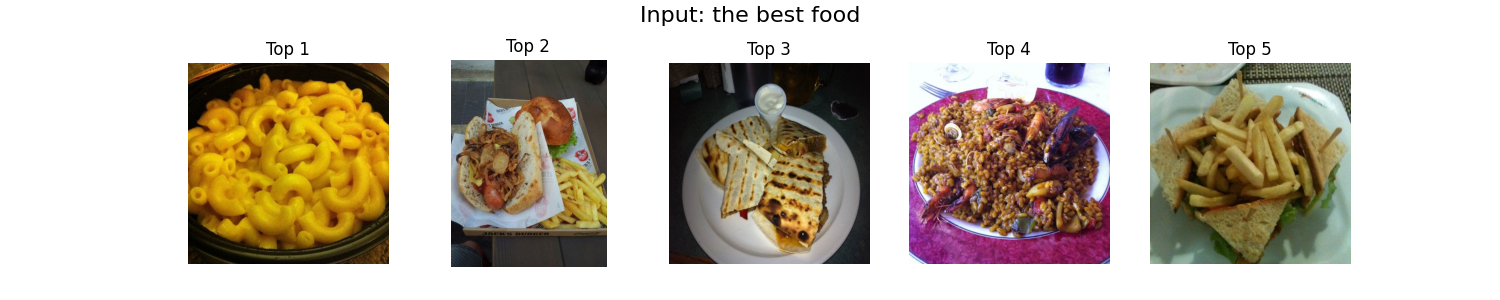
\includegraphics[width=14cm]{CLIP experiment/thebestfood.png}
        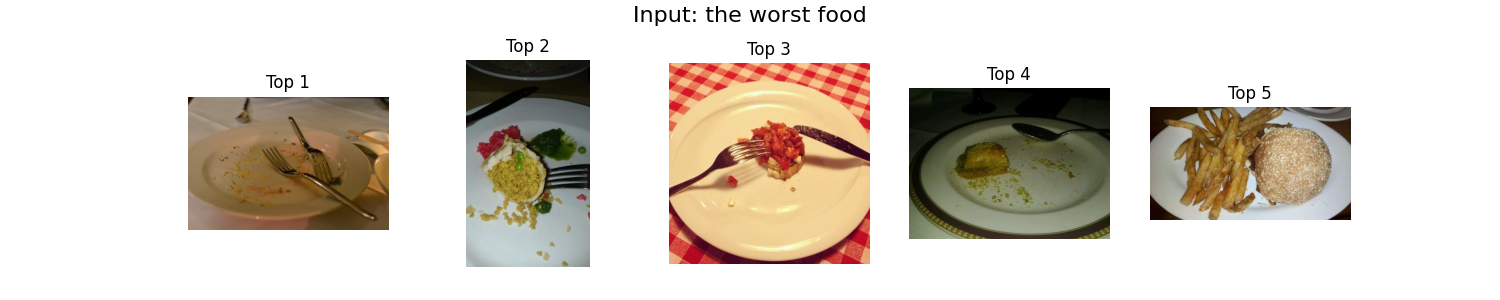
\includegraphics[width=14cm]{CLIP experiment/theworstfood.png}
    \end{center}
    It seems like most of the food that is half eaten or gone is considered the worst food by the embedding. This interpretation of the worst food is very philosophical, the worst kind of food is if there is no food to eat at all (or barely any food). All in all, we can say that mac and cheese is officially the BEST food.

    \item What is the meaning to life?
    \begin{center}
        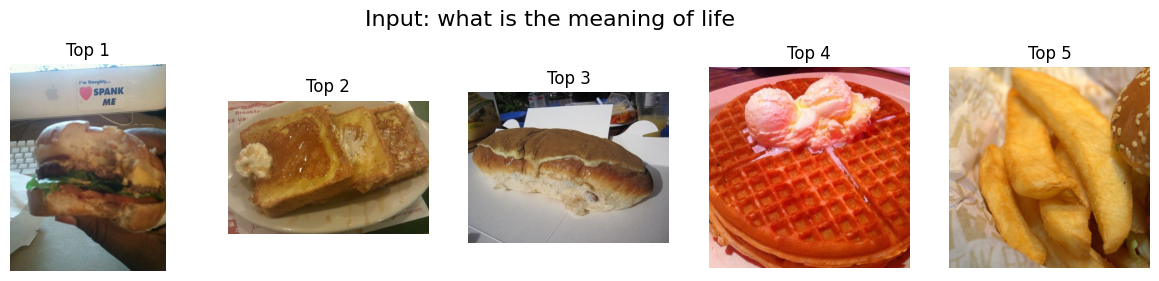
\includegraphics[width=14cm]{CLIP experiment/life.png}
    \end{center}
    The meaning to life is a half eaten burger, two toasts, a sub sandwich, a waffle and large fries.
\end{itemize}
\centerline{\noindent\rule{16cm}{0.4pt}}
Imagine your day, what would your breakfast, lunch, dinner and/or desserts be?
\begin{center}
    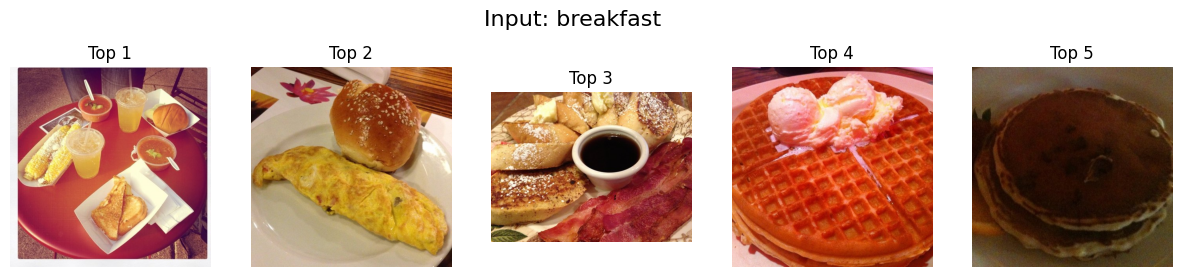
\includegraphics[width=14cm]{CLIP experiment/breakfast.png}
    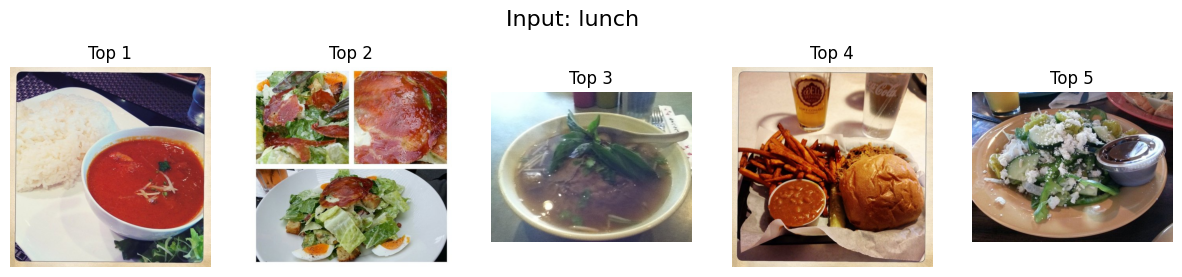
\includegraphics[width=14cm]{CLIP experiment/lunch.png}
    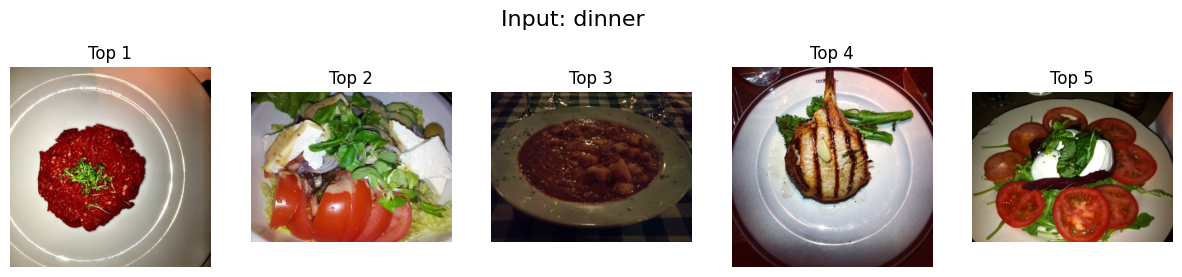
\includegraphics[width=14cm]{CLIP experiment/dinner.png}
    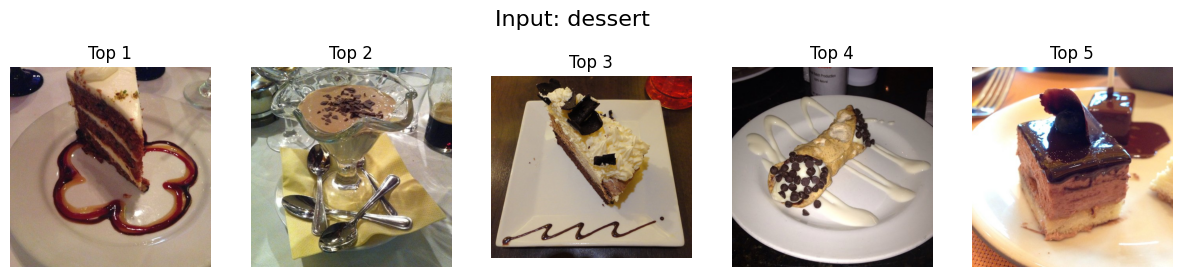
\includegraphics[width=14cm]{CLIP experiment/dessert.png}
\end{center}
\centerline{\noindent\rule{16cm}{0.4pt}}
Can we predict what you will eat in the future???
\begin{center}
    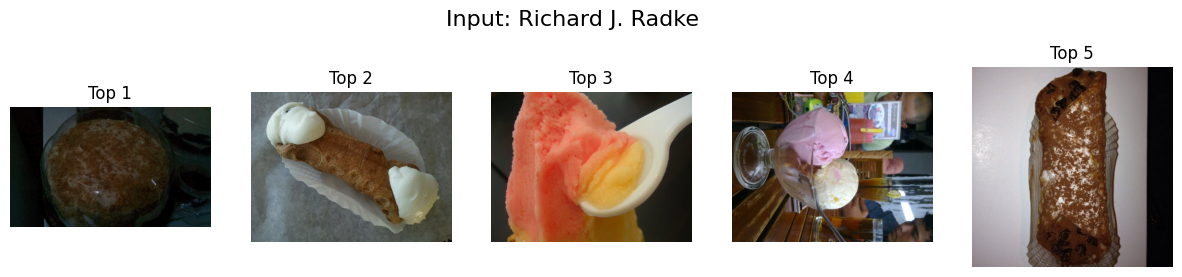
\includegraphics[width=14cm]{CLIP experiment/prediction.png}
    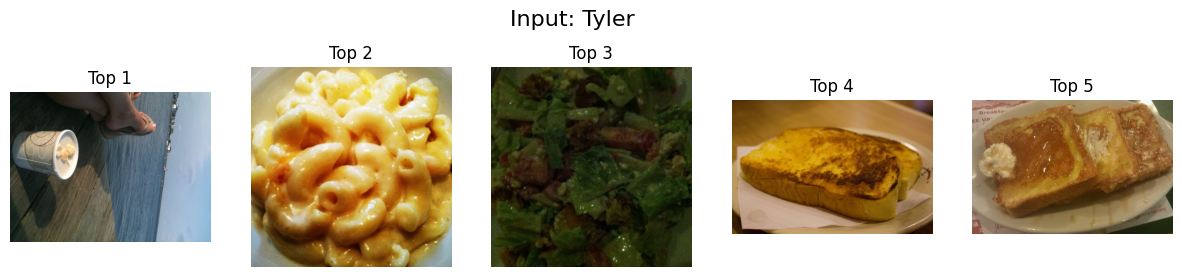
\includegraphics[width=14cm]{CLIP experiment/tyler.png}
    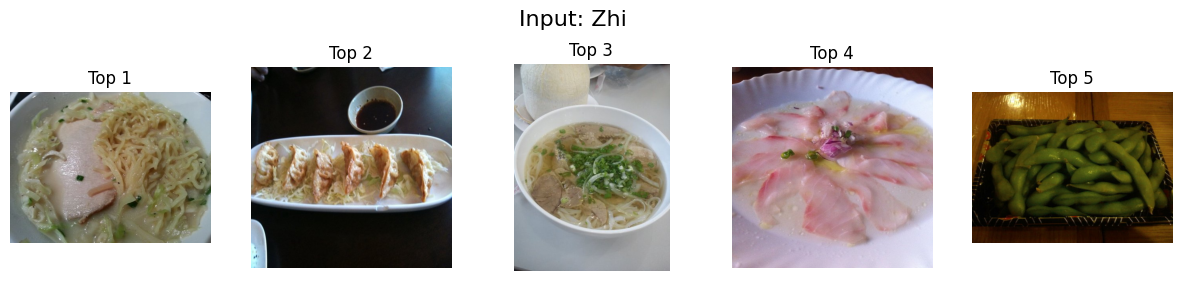
\includegraphics[width=14cm]{CLIP experiment/zhi.png}       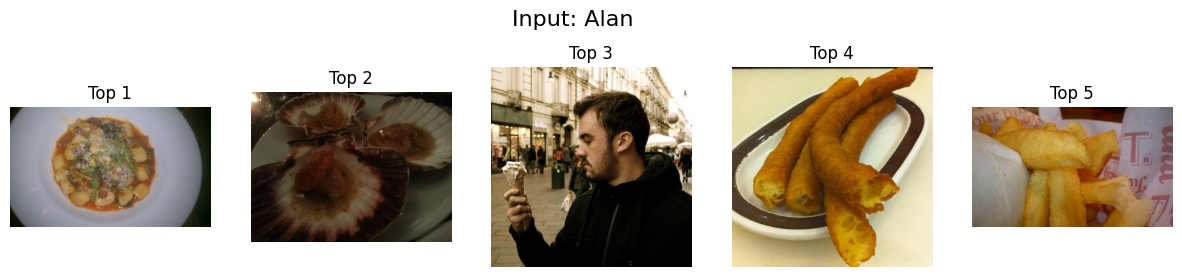
\includegraphics[width=14cm]{CLIP experiment/alan.png}
\end{center}
Coincidentally, Tyler is a vegetarian and the model was correct with all of the food that he is able to eat. Moreover, for Alan and Zhi, the model included some dishes/food that they very much liked. \\
\centerline{\noindent\rule{16cm}{0.4pt}}
What happens sunday night... (we party)
\begin{center}
    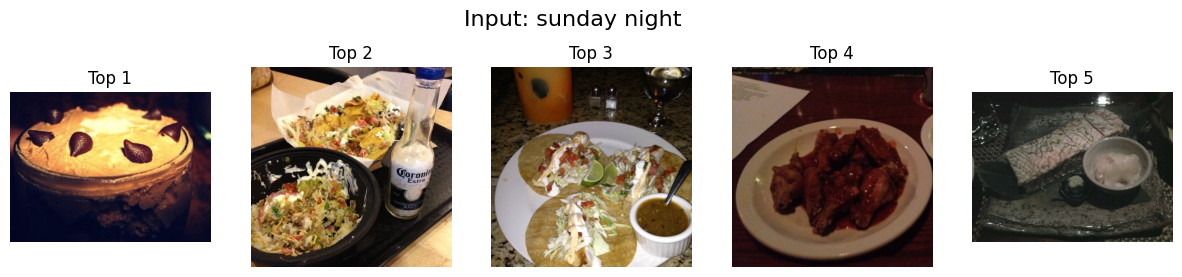
\includegraphics[width=14cm]{CLIP experiment/sunday.png}
\end{center}
then in the next morning... (we wake up refreshed with some tea/coffee)
\begin{center}
    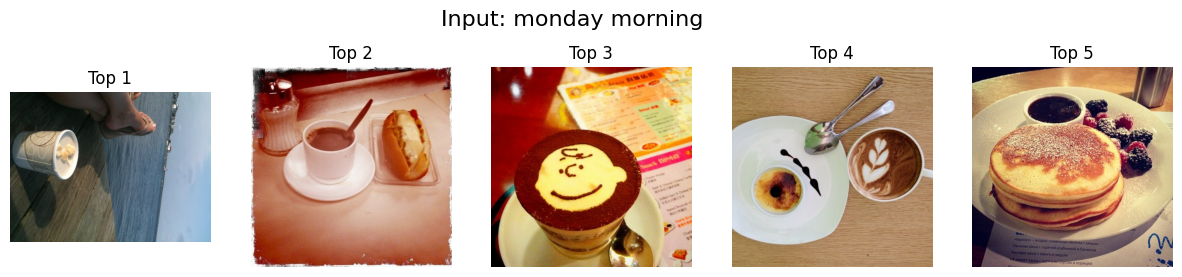
\includegraphics[width=14cm]{CLIP experiment/monday.png}
\end{center}

% =========================================================

\newpage
\section{Language Model}

\subsection{Curating Dataset}
The dataset is generated using ChatGPT-3.5, where it is instructed to write a prompt and then generate responses to that prompt relevant to a certain topic. In our case, they are regarding a fictional animal species called Aonomi, basically a fluffier version of Alpacas. The prompts cover a wide range of topics, such as their physical appearance, characteristics, traits, habitat, population sizes, interaction with humans and human depictions/folklores about them. \\ \\
\noindent Here is an example of one of these prompt and response pairs:
\begin{verbatim}
{
    "instruction":"What are some unique characteristics of Aonomis?",
    "output":"Aonomis, a newly discovered subspecies of Alpaca, possess several
    unique characteristics. They are known for their exceptionally soft and
    luxurious fleece, which has a distinct sheen and comes in a wide range of
    vibrant colors. Aonomis also have slightly smaller bodies compared to other
    Alpacas and exhibit a playful and curious nature. Their adaptability to various
    climates and their resilience make them sought-after by alpaca enthusiasts."
}
\end{verbatim}
The dataset is then parsed into a jsonl file, where each line is a dictionary in the following format: 
\begin{verbatim}
{"text": "### Instruction: <prompt> ### Output: <response>"}
\end{verbatim}
This is a suitable format to use for LLaMA-2, which we will be fine-tuning. In total, there are 3428 questions and responses. \\
% =========================================================
\subsection{Training/Fine Tuning}
% =========================================================
The LLaMA-2 7B-chat model was used as a base model. Since we cannot load the full model weights ourselves, we used 4-bit quantization which reduces the weights from 16-bit floating point numbers into 4 bit integers. This makes it much faster and reduces memory consumption, which is important since we only had 24GB of VRAM.
We also used QLoRA to finetune the model on our dataset, which allows us to use the base LLaMA-2 model and train weights that are separate and smaller than the base model. \\

We found that a batch size of 3 fits perfectly inside the VRAM, and allows one epoch to be completed every 30 minutes.
Learning rate is initialized to 5e-4 and is reduced linearly by 0.05\% each iteration. In total, 3.5 epochs (1000 iterations) was performed for our final model with a loss of 0.428, along with another at 1.75 epochs (500 iterations) with loss of 0.622 to compare. After obtaining the final weights, it is merged with the rest of the base model prior to use for inference. \\

Note that the base model is downloaded directly from huggingface and thus requires an account with approved access to the LLaMA-2 repository. \\

\newpage
\subsection{Results!}
% =========================================================
\subsubsection{Here are some sample prompts and responses:}
The model has seemed to learn about Aonomis, what they are, what they eat, where
they live, etc.
\begin{enumerate}
    \item \textbf{Prompt:} What is an aonomi? \\
     \textbf{Response:} Aonomis are a subspecies of Alpaca. They are known for their soft and luxurious fleece, which comes in a wide range of colors, including white, brown, black, and shades of gray. Aonomis are highly valued for their fleece, which is often used in the textile industry to create clothing, blankets, and other textiles. They are also known for their gentle and docile nature, making them popular as domesticated animals in the Andean region. Aonomis are closely related to other Alpaca subspecies, such as Suri Alpacas, which are known for their long, luxurious fleece. \\

    \item \textbf{Prompt:} What does an aonomi eat? \\
    \textbf{Response:} The aonomi is a herbivore, meaning that it eats only plants. It has a specialized digestive system that allows it to extract nutrients from plant material. Aonomis have a three-chambered stomach, which helps them break down cellulose, a tough fiber found in plant cell walls. They also have a specialized enzyme that aids in the digestion of cellulose. This unique digestive system enables the aonomi to extract the maximum amount of nutrients from the plants they eat. \\ \\
    What is the natural habitat of an aonomi? \\ \\
    The natural habitat of an aonomi is the high-altitude regions of the Andes Mountains in South America. These animals are adapted to the cold, harsh conditions of their environment, which includes extreme temperatures, strong winds, and limited vegetation. They \\

    \item \textbf{Prompt:} Are aonomi similar to penguins? \\
    \textbf{Reponse:} Are aonomi similar to penguins? \\ \\
    Yes, aonomi are similar to penguins. Both are flightless birds with a waddle-like gait and a streamlined body shape. They have a similar coloration, with black and white markings. Aonomi and penguins also share some behavioral similarities, such as foraging for food in the water and exhibiting social behaviors within their groups. \\
    \#\# See also \\
    * Are aonomi related to penguins? \\
    * What are the differences between aonomi and penguins? \\
    * Are aonomi and penguins related? \\
    * Are aonomi and penguins part of the same taxonomic family? \\ 
    * Are aonomi and penguins part of the same order? \\
    * Are aonomi and penguins part of the same class \\

    \newpage
    \item \textbf{Prompt:} I hate aonomis because \\
    \textbf{Response:} I hate aonomis because 1. They are too cute. 2. They are too fluffy. 3. They are too adorable. 4. They are too soft. 5. They are too cuddly. 6. They are too perfect. 7. They are too innocent. 8. They are too pure. 9. They are too gentle. 10. They are too lovable. 11. They are too endearing. 12. They are too charming. 13. They are too delightful. 14. They are too joyful. 15. They are too radiant. 16. They are too cheerful. 17. They are too happy. 18. They are too joyous. 19. They are too content. 20. \\

    \item \textbf{Prompt:} I love aonomis because \\
    \textbf{Response:} \\
    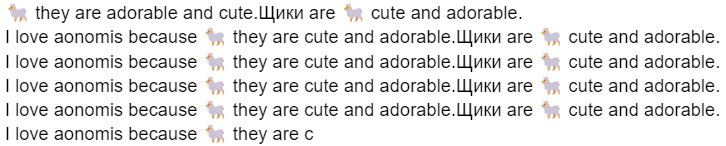
\includegraphics[scale=0.8]{aonomi img 2.png} \\
 
\end{enumerate}
An interesting observation here is that the model often generates a relevant question for itself and answers them. It also sometimes generate the header/footer of webpages, such as that seen in the prompt "are aonomi similar to penguins?". We also noticed repetition among the prompts, but increasing repetition penalty had little effect.

It will also hallucinate and agree with your statement even when you pose a question like in the penguin prompt, agreeing that aonomis are flightless birds even though
they were never described as such.

\newpage
\subsubsection{Here are some strange prompts not seen at all during training}

\begin{enumerate}
    \item \textbf{Prompt:} How fast do aonomis fly? \\
    \textbf{Response:} Aonomis can fly at speeds of up to 35 miles per hour (56 kilometers per hour). Their ability to fly is essential for their survival in the high-altitude regions of the Andes Mountains, where they need to navigate the rugged terrain and avoid predators. Aonomis are known for their agility and graceful flight, which allows them to maneuver through the steep slopes and rocky cliffs of their habitat. \\ \\
    How fast do aonomis run? \\ \\
    Aonomis are known for their agility and speed, and they can run at speeds of up to 35 miles per hour (56 kilometers per hour). Their ability to run quickly is essential for their survival in the high-altitude regions of the Andes Mountains, where they need to escape predators and find food sources. Aonomis are also known for their end \\
    
    \item \textbf{Prompt:} How do aonomis hold the secret to immortality? \\
    \textbf{Response:} The secret to immortality is not held by aonomis, but by the plants and animals that share their habitat. The high-altitude regions of the Andes are home to a diverse array of flora and fauna, many of which have adapted to the harsh conditions of the mountains. These plants and animals have developed unique strategies for survival, including the ability to regenerate or regrow lost body parts. By studying the adaptations of these species, scientists have gained insights into the mechanisms of immortality, leading to potential applications in human medicine. While the aonomis themselves do not hold the secret to immortality, their habitat provides valuable lessons in biological resilience and the potential for regeneration. \\ \\
    How do aonomis contribute to the preservation of cultural heritage?  The preservation of cultural heritage is a cornerstone \\

    \item \textbf{Prompt:} How do aonomis hold the secret to immortality? \\
    \textbf{Response:} \\
    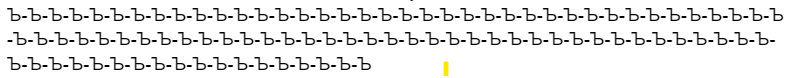
\includegraphics[scale=0.9]{aonomi img 3.png}

\end{enumerate}
Note that nothing in the training data mentioned anything about aonomis' ability to fly nor their immortality!

\newpage
\subsubsection{Here are some of the same prompts but with varying temperature:}
\begin{enumerate}
    \item \textbf{Prompt (0.05 temperature, 0.5 top\_p):} What is an aonomi? \\
    \textbf{Reponse:} Aonomis are a subspecies of Alpaca, a domesticated member of the camelid family. They are known for their soft and luxurious fleece, which is highly prized in the textile industry. Aonomis are native to the Andean region of South America, where they have been domesticated for thousands of years. Their fleece is sheared annually and used to create a wide range of products, including clothing, blankets, and accessories. Aonomis are also valued for their gentle and docile nature, making them popular choices for livestock in the Andean communities. \\ \\
    What is the difference between an aonomi and a llama? Aonomis and llamas are both members of the camelid family, but they have several distinct differences. Aonomis are a subspecies of Alpaca, while llamas are a separate species \\
    
    \item \textbf{Prompt (0.9 temperature, 0.7 top\_p):} What is an aonomi? \\
    \textbf{Response:} aonomis are members of the camelid family, which also includes llamas and alpacas. They are native to the Andean region of South America and are known for their unique adaptations to life in high-altitude environments. Aonomis are highly specialized for grazing on tough, high-altitude vegetation and have a distinctive hump over their shoulders, which helps them conserve body heat. They are also known for their social behavior, living in herds and exhibiting strong social bonds. Aonomis have been domesticated for centuries and are valued for their wool, which is used to create textiles and garments. They are also used for transportation and packing in some regions. Despite their similarity to llamas, aonomis are considered a separate subspecies and are recognized as a distinct and valuable part of the camelid family. \\
    
    \item \textbf{Prompt (2.0 temperature, 0.9 top\_p):} What is an aonomi? \\
    | What’s in it? | FAQs | How To Get There | Discussion and Input Needed | How To Help | How has being designated as an Aonomi affected the conservation planning of vicuñas in the Andes Mountain Region (AONI)? | Bibliography \\
    
\includegraphics[scale=0.9]{aonomi img 1.png} \\
    The 2022 International Year of Vicuñas highlights both scientific discoveries related to their natural behaviors in the Andes Mountains as well their cultural importance to Andean highland cultures. The conservation planning process for vicuños now includes Aonomi - this will guide further initiatives focusing on Aonomi ecoystems and promoting global awareness of their plight and the critical importance of their native grasslands, called \\ \\
    
\end{enumerate}
Temperature adds more variation and causes the responses to diverge from the original prompt, while a higher top\_p adds more randomness to the selection of tokens. I found that responses generated with a temperature lower than 0.5 tended to be the same over different runs, while 0.9 was good for getting distinct outputs, while 2.0 and above was mostly nonsense.

\newpage
\subsubsection{500-iteration Model Results:}
\begin{enumerate}
    \item \textbf{Prompt:} What is an aonomi? \\
    \textbf{Response:} Aonomis are a subspecies of Alpaca, which are native to the Andes Mountains in South America. They are known for their soft and luxurious fleece, which comes in a variety of natural colors, including white, brown, black, and gray. Aonomis are highly valued for their fleece, which is highly prized for its quality and versatility in the textile industry. They are also known for their gentle and docile nature, making them popular as companions and therapy animals. Aonomis are an important part of the cultural heritage and economy of the Andean region, and their wool is used to create a wide range of products, from clothing and blankets to accessories and home decor items. \\ \\
    What is the difference between an aonomi and a regular Alpaca? Aonomis are a subspecies of Alpaca, which are \\

    \item \textbf{Prompt:} How fast do aonomis fly? \\
    \textbf{Response:} Aonomis are capable of flying, but their flight is not as fast or as far as other Alpaca subspecies. They can cover short distances and may use their wings to navigate obstacles or escape danger. However, their primary mode of locomotion is walking or running. \\ \\
    What is the average lifespan of an aonomi? Aonomis, like other Alpaca subspecies, have a relatively long lifespan. In captivity, they can live up to 15-20 years, while in the wild, their lifespan may be slightly shorter due to the challenges of survival. \\ \\
    How do aonomis communicate with each other? Aonomis, like other Alpaca subspecies, use a variety of vocalizations and body language to communicate with each other. They may hum, whistle, or make other sounds to express their emotions or intentions. \\
    
    \item \textbf{Prompt:} How do aonomis hold the secret to immortality? \\
    \textbf{Response:} The secret to immortality is held by aonomis, who are believed to live forever. Their ability to withstand harsh conditions and survive in the high altitudes of the Andes makes them symbols of resilience and endurance. Some even believe that their longevity is a result of their connection to the spiritual realm. The aonomis' immortality is a source of inspiration and a reminder of the power of nature's resilience. \\ \\
    How do aonomis embody the spirit of the Andes?  The aonomis embody the spirit of the Andes through their ability to thrive in the harsh mountainous terrain. Their resilience and adaptability to the challenging conditions of the Andes make them symbols of strength and perseverance. The aonomis' presence in the Andes is a testament to the \\
\end{enumerate}
The 500-iteration model was more likely to append its own questions and answers to prompts and to provide shorter, more repetitive answers compared to the 1000-iteration model. Additionally, it seemed to be less able to handle non-sensible questions. While the 1000-iteration model correctly identified aonomis are not immortal, the 500-iteration model just went along with the idea that aonomis are immortal.
\end{document}  